%\documentclass[xcolor=dvipsnames, handout]{beamer} %This turns on handouts
\documentclass[xcolor=dvipsnames]{beamer} %This is normal slide mode

% Color and font packages
\usepackage{xcolor,colortbl,lmodern}
\usepackage[T1]{fontenc}
\usepackage[english]{babel}

% Setup the theme
\usetheme{CambridgeUS}
\setbeamertemplate{items}[ball]
\setbeamertemplate{navigation symbols}{}
\setbeamercolor{item projected}{bg=red}

% URL, verbatim, and math packages
\usepackage{fancyvrb,alltt,hyperref,url}
\usepackage{amsmath,amssymb}

% More beamer specific packages for things like animations, table layouts, etc.
\usepackage{dcolumn,url,enumerate,verbatim, epsfig,bbm,calc,color,ifthen,capt-of,animate}
\usepackage{appendixnumberbeamer}

% Figure and code packages + configuration for code
\usepackage{graphicx,listings}
\lstset{
  basicstyle=\small\ttfamily,
  language=[latex]tex,
  columns=flexible,
  commentstyle=\color{blue},
  breaklines=true
}

% Citation management package
\usepackage{natbib}

% Document information and title page
\title{Introduction to \LaTeX}
\author[Kaplan]{Adam Kaplan\\akapl@mit.edu}
\date[Sept 30, 2020]{September 30, 2022\\ \vspace{1em} {\footnotesize These slides build on materials from
    previous years by Emilia Simison, Dan de Kadt, Elizabeth Dekeyser, Nina McMurry, Weihuang Wong, and Guillermo Toral, and on \href{https://tobi.oetiker.ch/lshort/lshort.pdf}{``The Not So Short Introduction to \LaTeX{}''}.}}

% Progress slide before each section
\AtBeginSection[]
{
  \begin{frame}
    \frametitle{Where we are}
    \tableofcontents[currentsection]
  \end{frame}
}


%-----------------------------------------------------------------------------
\begin{document}
%-----------------------------------------------------------------------------

\frame{\titlepage}

%-----------------------------------------------------------------------------

\begin{frame}
  \frametitle{What we'll cover today}
  \tableofcontents
\end{frame}

\section{Introduction}

\begin{frame}
  \frametitle{What's \LaTeX?}
  \begin{itemize}
    \item \LaTeX{} is a typesetting system that produces high-quality documents --
          anything from letters, papers, dissertations, posters, slides (like
          these ones), resumes, etc. \pause
          % There are many readily-available layouts that you can download for free from the Internet.
    \item \LaTeX, unlike Word or other normal word processor, is not a WYSIWYG (``what you see is what
          you get'') system. Using it requires a bit of a change of mindset. \pause
    \item In \LaTeX, you write the code, and then the software compiles or creates
          the document as a PDF file.  In other words, content entry takes place separately from formatting.
          \pause
    \item Like \texttt{R}, there are hundreds of add-ons available that you can use.
  \end{itemize}
\end{frame}


\begin{frame}
  \frametitle{Why use \LaTeX?}
  \begin{itemize}
    \item \LaTeX{} makes math much easier to write and to display well: \pause
          $$ Y_{i} = \alpha + X_i\beta + \varepsilon_i $$ \pause
          $$ f(y) = \frac{1}{y!\Gamma(\alpha)\beta^\alpha}\int_{0}^{\infty} \mu^{y+\alpha-1} \exp\left(-\mu\left[1+\frac{1}{\beta}\right]\right)\,d\mu $$ \pause
    \item \LaTeX{} works well with \texttt{R}: you can easily input plots and tables
          from \texttt{R}, and you can even write \LaTeX{} documents directly from R \pause
    \item \LaTeX{} makes it easy to manage large documents, with references
          and bibliography, cross-references and links inside the document, etc. \pause
    \item \LaTeX{} is used widely in the scientific community, and some people see it as a signal of credibility
  \end{itemize}
\end{frame}

\begin{frame}
  \frametitle{Things to keep in mind about \LaTeX}
  \begin{itemize}
    \item \LaTeX{} is a skill that takes some effort -- and patience -- to
          build. \pause
    \item Grad school gives you the time and incentives to do so -- invest
          some effort, and it'll pay off. \pause
    \item \LaTeX{} is a good tool for some purposes -- once you master it,
          it becomes very easy to use, and it allows you to do cool things
          that would be harder to do without \LaTeX. \pause
    \item \LaTeX{} is not so good for other purposes, like spellchecks or
          review tools, although you can also do those in \LaTeX. \pause
    \item \LaTeX{} is a tool -- the more you have, the better.
  \end{itemize}
\end{frame}

%-----------------------------------------------------------------------------

\section{\LaTeX{} Language}

\begin{frame}[fragile]
  \frametitle{Text, formulas, and commands}

  Consider the following sentence:

  \begin{center}
    A ``source file'' has text, formulas (e.g. $\sqrt{5}$), and \emph{commands to} \LaTeX
  \end{center}
  \pause
  Here's the source for the above sentence:

  \begin{lstlisting}
  A ``source file'' has text, formulas (e.g. $\sqrt{5}$), and
  \emph{commands to} \LaTeX
  \end{lstlisting}
  \pause
  It's made up of:

  \begin{itemize}
    \item text: \verb+A ``source file'' has text, formulas (e.g....+
    \item formula: \verb+$\sqrt{5}$+
    \item more text: \verb+), and+
    \item commands: \verb+\emph{commands to} \LaTeX+
  \end{itemize}

\end{frame}

\begin{frame}
  \frametitle{Commands \& spaces}
  Commands:
  \begin{itemize}
    \item \LaTeX{} commands start with \textbackslash{} and continue with letters or
          with one non-letter (e.g. \texttt{\textbackslash begin\{\}}, \texttt{\textbackslash end\{\}}, \texttt{\textbackslash textbf\{\}}, \texttt{\textbackslash dots}, \texttt{\textbackslash \&}).
    \item Many commands have a ``starred'' version, where the name of the
          command is followed by ``*''. This usually tells \LaTeX{} to omit
          numbering (e.g. \texttt{\textbackslash section*} means do not number this section).
  \end{itemize}
  \pause
  White spaces:
  \begin{itemize}
    \item ``Whitespace'' characters (whether one space, one tab, or several
          spaces/tabs) are all treated as one space.
    \item An empty line or multiple
          empty lines are all treated as an empty line (which ends a
          paragraph).
    \item Spaces after commands are ignored, so it's good to write
          \texttt{\{\}} after them: \texttt{\textbackslash LaTeX\{\}}.
    \item You can insert a line break with \texttt{\textbackslash
            \textbackslash} or \texttt{\textbackslash newline}. For a page
          break, use \texttt{\textbackslash newpage}.
  \end{itemize}
\end{frame}

\begin{frame}
  \frametitle{Reserved characters}
  There are some ``reserved'' characters in \LaTeX:
  \begin{itemize}
    \item $\backslash$ says: read text following this as an operation.
    \item $\$ $  says: open an inline math environment. Put another to close it.
    \item $\% $ says: ignore text that follows -- allows you to comment your code.
    \item $\& $ says: position this to line up with other position indicators.
    \item $\{   \}$ says: group these items.
    \item \_{} says: write what follows as a subscript.
    \item \^{} says: write what follows as a superscript.
  \end{itemize}
  If you actually want to print these characters, you need to use
  ``\textbackslash{}'' before them (e.g. \texttt{\textbackslash \&}), or \texttt{\textbackslash textbackslash} for the backslash.
\end{frame}

%-----------------------------------------------------------------------------

\section{Setting up a \LaTeX{} document}

\begin{frame}[fragile]
  \frametitle{Key components of a \LaTeX{} document}
  \LaTeX{} documents typically include the following components:
  \begin{itemize}
    \item Preamble: declares the type of the document, gives its
          parameters, and loads packages
    \item Titling: declares the document's title, author(s), and date.
    \item Document itself, which may include a title page, sections, subsections,
          bibliography, etc.
  \end{itemize}
  \pause
  \vspace*{0.5cm}
  A minimal \LaTeX{} document includes the following code (written in a \texttt{.tex} file)
  \begin{lstlisting}
  \documentclass[options]{class}
  \usepackage[options]{packages}
  \begin{document}
  Your document.
  \end{document}
  \end{lstlisting}
\end{frame}

\begin{frame}
  \frametitle{\LaTeX{} mechanics}
  Here are the steps you usually take to create a document with \LaTeX{}:
  \pause
  \begin{itemize}
    \item Write in your \texttt{.tex} file, and save it. \pause
    \item Compile the \LaTeX{} file into a PDF by pressing the
          corresponding button in the TeX software you use. Sometimes you need to do
          this several times, especially if you have a bibliography
          in the document. \pause
    \item A new \texttt{.pdf} file (and a number of auxiliary files terminating in
          \texttt{.aux}, \texttt{.out}, \texttt{.toc}, etc.) will appear in the same folder as your \texttt{.tex} file. \pause
    \item It is useful to compile your PDF from time to time as you write,
          to make sure it's compiling correctly.
    \item You can use your Tex PDF reader side by side, so you can see in real time what your output looks like (this is what TexMaker does).
  \end{itemize}
\end{frame}


\begin{frame}
  \frametitle{Let's practice!}
  Let's start by building a minimum article document.
  \begin{itemize}
    \item Open a \texttt{.tex} file and fill it up.
          \begin{itemize}
            \item Give it a document class e.g. \texttt{article}. \footnotesize{(You can also try \texttt{report}, and insert optional arguments, e.g. \texttt{letterpaper}, \texttt{a4paper}, \texttt{10pt}, \texttt{12pt}. You can insert multiple arguments, separated by a comma.)}
            \item Fill in the titling information.
          \end{itemize}
          \pause
    \item Add some text.
          \begin{itemize}
            \item Try structuring your text with sections, by using
                  \texttt{\textbackslash section\{Section~name\}}. You can also
                  use  \texttt{\textbackslash subsection\{\}} and
                  \texttt{\textbackslash subsubsection\{\}}.
            \item You can also add some \texttt{\textbackslash footnote\{\}}.
          \end{itemize}
    \item When you're ready, save the file and compile it.
    \item Open the resulting PDF file.
  \end{itemize}
\end{frame}

\begin{frame}
  \frametitle{An empty template for a \texttt{.tex} file}
  \begin{center}
    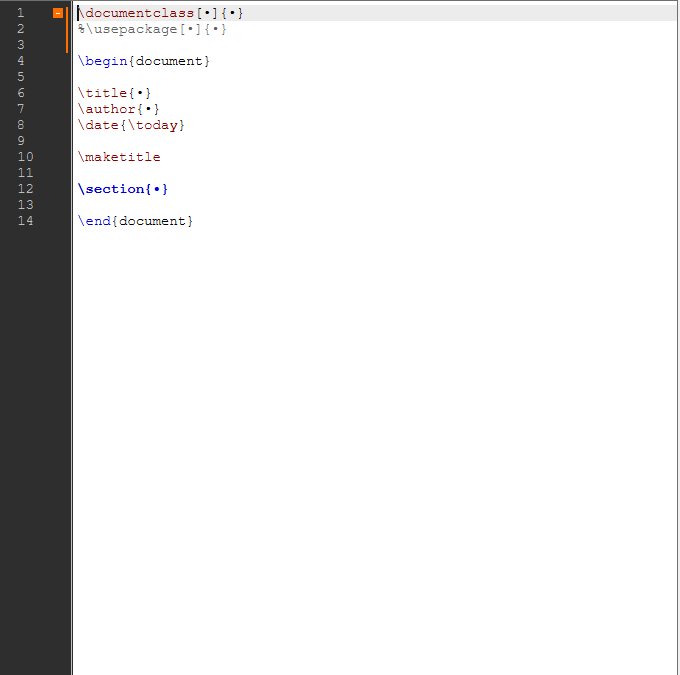
\includegraphics[scale=0.7]{figures/template_image.png}
  \end{center}
\end{frame}

\begin{frame}
  \frametitle{A simple \texttt{.tex} file}
  \begin{center}
    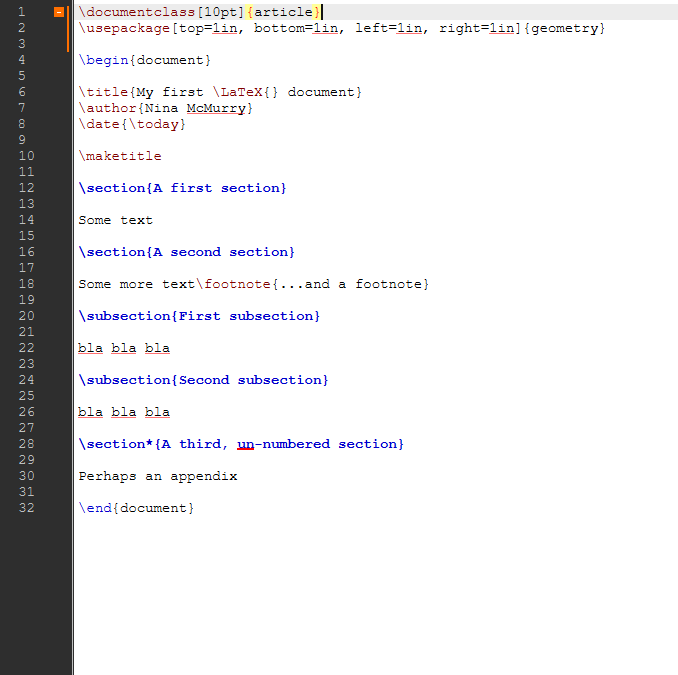
\includegraphics[scale=0.7]{figures/template_image_filled.png}
  \end{center}
\end{frame}

\begin{frame}
  \frametitle{The resulting PDF file}
  \begin{center}
    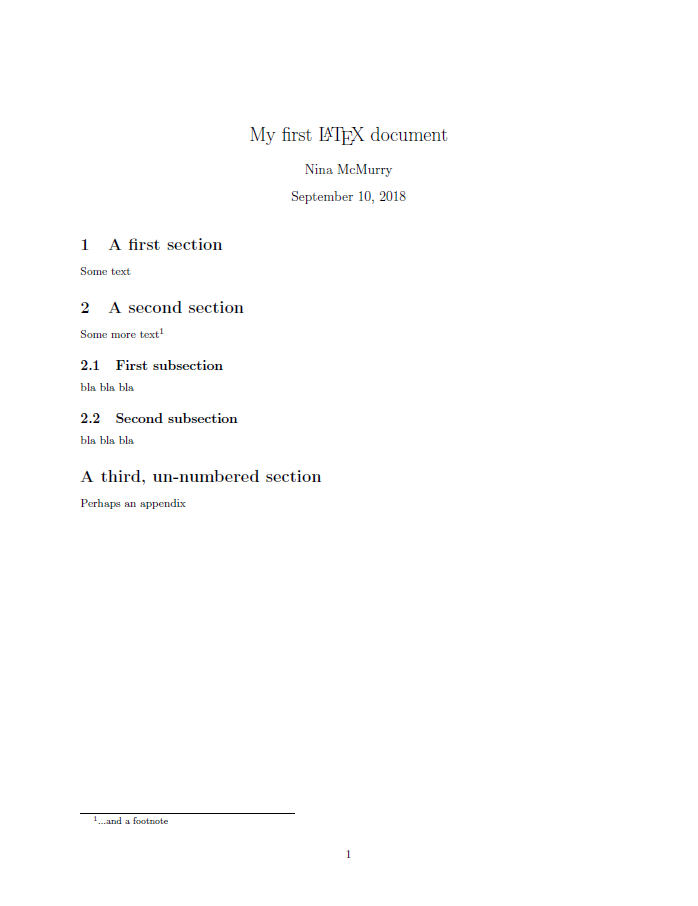
\includegraphics[scale=0.5]{figures/template_image_result.png}
  \end{center}

\end{frame}

%-----------------------------------------------------------------------------

\section{\LaTeX{} environments \& commands}

\begin{frame}[fragile]
  \frametitle{What's an environment?}
  \LaTeX\ uses ``environments'' to format content:
  \begin{itemize}
    \item When you \verb+\begin{environment}+ a set of rules is applied to the content that appears \textit{within that environment}.
    \item When you \verb+\end{environment}+ those rules no longer apply.
    \item Environments can be embedded within environments.
    \item We have already used one. Do you remember which one?
          \pause
    \item Yes! The biggest environment is the \texttt{document} environment, which bounds the entire document you make.
    \item Environments can be used for lists, for including figures, equations, tables, plots, text in different sizes or alignments, abstracts, long quotes, etc.
  \end{itemize}
\end{frame}

\begin{frame}[fragile]
  \frametitle{Using an environment}
  Here's how you can use a basic text environment, \texttt{itemize}:
  \begin{lstlisting}
  Some countries in the Southern Cone
  \begin{itemize}
  \item Argentina
  \item Chile
  \item Brazil
  \end{itemize}
  \end{lstlisting}
  \pause
  Which produces the following: \\
  Some countries in the Southern Cone
  \begin{itemize}
    \item Argentina
    \item Chile
    \item Brazil
  \end{itemize}
  \pause
  If we substituted \texttt{enumerate} for \texttt{itemize} (make sure to use the
  \texttt{enumitem} package!) we'd get a numbered list.
\end{frame}


\begin{frame}[fragile]
  \frametitle{Let's practice!}
  Now practice creating and filling an \texttt{enumerate} environment within
  your practice \texttt{.tex} file:
  \begin{itemize}
    \item Load the \texttt{enumitem} package in the file's preamble.
    \item Begin an \texttt{enumerate} environment. It takes some options (e.g., \verb+[label = (\arabic*)]+ or \verb+[label = \alph*.]+)
    \item Create \texttt{item}s.
    \item End the \texttt{enumerate} environment.
    \item Optional: Wrap the whole \texttt{enumerate} environment in a \texttt{center} environment.
  \end{itemize}
\end{frame}


\begin{frame}[fragile]
  \frametitle{Math environments}
  Let's now add math to our document:
  \begin{enumerate}
    \item Load the \texttt{amsmath} and \texttt{amssymb} packages in your document's preamble.
    \item Begin an \texttt{align*} environment
    \item Type in some math: \newline \texttt{Y$\_$i \alert{\&}= $\backslash$alpha + $\backslash$beta x$\_$i + $\backslash$varepsilon$\_$i}
    \item End the line with \texttt{\textbackslash\textbackslash{}} to separate lines.
    \item Type a second line: \newline \texttt{Y$\_$i - $\backslash$varepsilon$\_$i \alert{\&}= $\backslash$alpha + $\backslash$beta x$\_$i}
    \item End the \texttt{align*} environment.
  \end{enumerate}

  This produces a set of aligned equations (what if you omit the \texttt{*} from \texttt{align*}?):
  \begin{align*}
    Y_i                 & = \alpha + \beta x_i + \varepsilon_i \\
    Y_i - \varepsilon_i & = \alpha + \beta x_i
  \end{align*}
\end{frame}

\begin{frame}[fragile]
  \frametitle{Math environments}
  We can also create a \textit{non-aligned} math environment using \texttt{\$} and \texttt{\textbackslash[}.\pause
  \begin{itemize}
    \item \texttt{\$...\$} creates in-line math, \texttt{\textbackslash[...\textbackslash]} creates displayed math.
    \item Example of in-line math with \texttt{\$}: writing \verb|$\sum_{i=1}^{3}i = 1 + 2 + 3$| will produce $\sum_{i=1}^{3}i = 1+ 2 + 3$.
    \item Example of displayed math with \texttt{\textbackslash[}: writing
          \verb|\[\sum_{i=1}^{3}i = 1 + 2 + 3\]| will produce
          \[\sum_{i=1}^{3}i = 1+ 2 + 3\]
  \end{itemize}
  If you want display-style, numbered equations, but you don't want to align
  them, or you're writing only one equation, you can use the environment \texttt{equation}.
\end{frame}

\begin{frame}[fragile]
  \frametitle{Some math symbology}
  \begin{center}
    \footnotesize
    \begin{tabular}{lll}
      \hline
      \hline
      \LaTeX{} code                           & Output                               & What to use it for     \\
      \hline                                                                                                  \\
      \verb|a+b,a \times b,a \cdot b|         & $a+b, a \times b, a \cdot b$         & Arithmetic             \\[3pt]
      \verb|y_{ijk},y^{ijk}|                  & $y_{ijk}, y^{ijk}$                   & Subscript, superscript \\[3pt]
      \verb|\sqrt{x},\sqrt[y]{x}|             & $\sqrt{x},\sqrt[y]{x}$               & Square root, y-th root \\[3pt]
      \verb|\frac{x}{y}|                      & $\frac{x}{y}$                        & Fractions              \\[3pt]
      \verb|\left(\frac{x}{y}\right)|         & $\left(\frac{x}{y}\right)$           & Delimiters             \\[3pt]
      \verb|\binom{n}{n-k}|                   & $\binom{n}{n-k}$                     & Binomial coefficients  \\[3pt]
      \verb|\alpha|                           & $\alpha$                             & Greek letters          \\[3pt]
      \verb|\exp,\log,\Pr|                    & $\exp,\log,\Pr$                      & Operators              \\[3pt]
      \verb|\bar{X},\hat{\beta},\widehat{XY}| & $\bar{X}, \hat{\beta}, \widehat{XY}$ & Accents                \\[3pt]
      \verb|\mathcal{R},\mathbb{E}|           & $\mathcal{R},\mathbb{E}$             & Math fonts             \\[3pt]
      \hline
      \hline
    \end{tabular}
  \end{center}
\end{frame}

\begin{frame}[fragile]
  \frametitle{More math symbology}
  \begin{center}
    \footnotesize
    \begin{tabular}{lll}
      \hline
      \hline
      \LaTeX{} code                       & Output                                                                   & What to use it for \\
      \hline                                                                                                                              \\
      \verb|\sum_{k=0}^{n-1}a r^k|        & $\sum_{k=0}^{n-1}a r^k,\displaystyle\sum_{k=0}^{n-1}a r^k$               & Sums               \\[15pt]
      \verb|\int_0^{\infty}e^{-x}\,dx|    & $\int_0^{\infty}e^{-x}\,dx,\displaystyle\int_0^{\infty}e^{-x}\,dx$       & Integrals          \\[15pt]
      \verb|\lim_{n \to \infty}\bar{X}_n| & $\lim_{n \to \infty}\bar{X}_n,\displaystyle\lim_{n \to \infty}\bar{X}_n$ & Limits             \\[15pt]
      \hline
      \hline
    \end{tabular}
  \end{center}

  See \url{http://detexify.kirelabs.org/classify.html} if you need to look up a symbol.\\
  And nerdiness save Mathpix!

\end{frame}

\begin{frame}[fragile]
  \frametitle{\LaTeX{} commands}
  Commands are another way of taking in content and create output:
  \begin{itemize}
    \item No need to use \verb+\begin+ and \verb+\end+ with commands. Instead you simply use \verb+\command{your input}+.
    \item We've already used a couple, like \verb+\section+ or \verb+\item+.
    \item Some commands take options in square brackets: \verb+\command[options]{your input}+
  \end{itemize}

  % We can use commands to include graphics in our document:
  % \begin{enumerate}
  % \item Load the \texttt{graphicx} package.
  % \item Begin a ``center'' environment so the graph shows centered.
  % \item Use the ``includegraphics'' command. It takes some options and some arguments:
  % \item Options in square brackets: [scale = .5]
  % \item A filename in curly braces: \{graph.pdf\}
  % \item End the ``center'' environment.
  % \end{enumerate}
\end{frame}


\begin{frame}
  \frametitle{Some useful commands}
  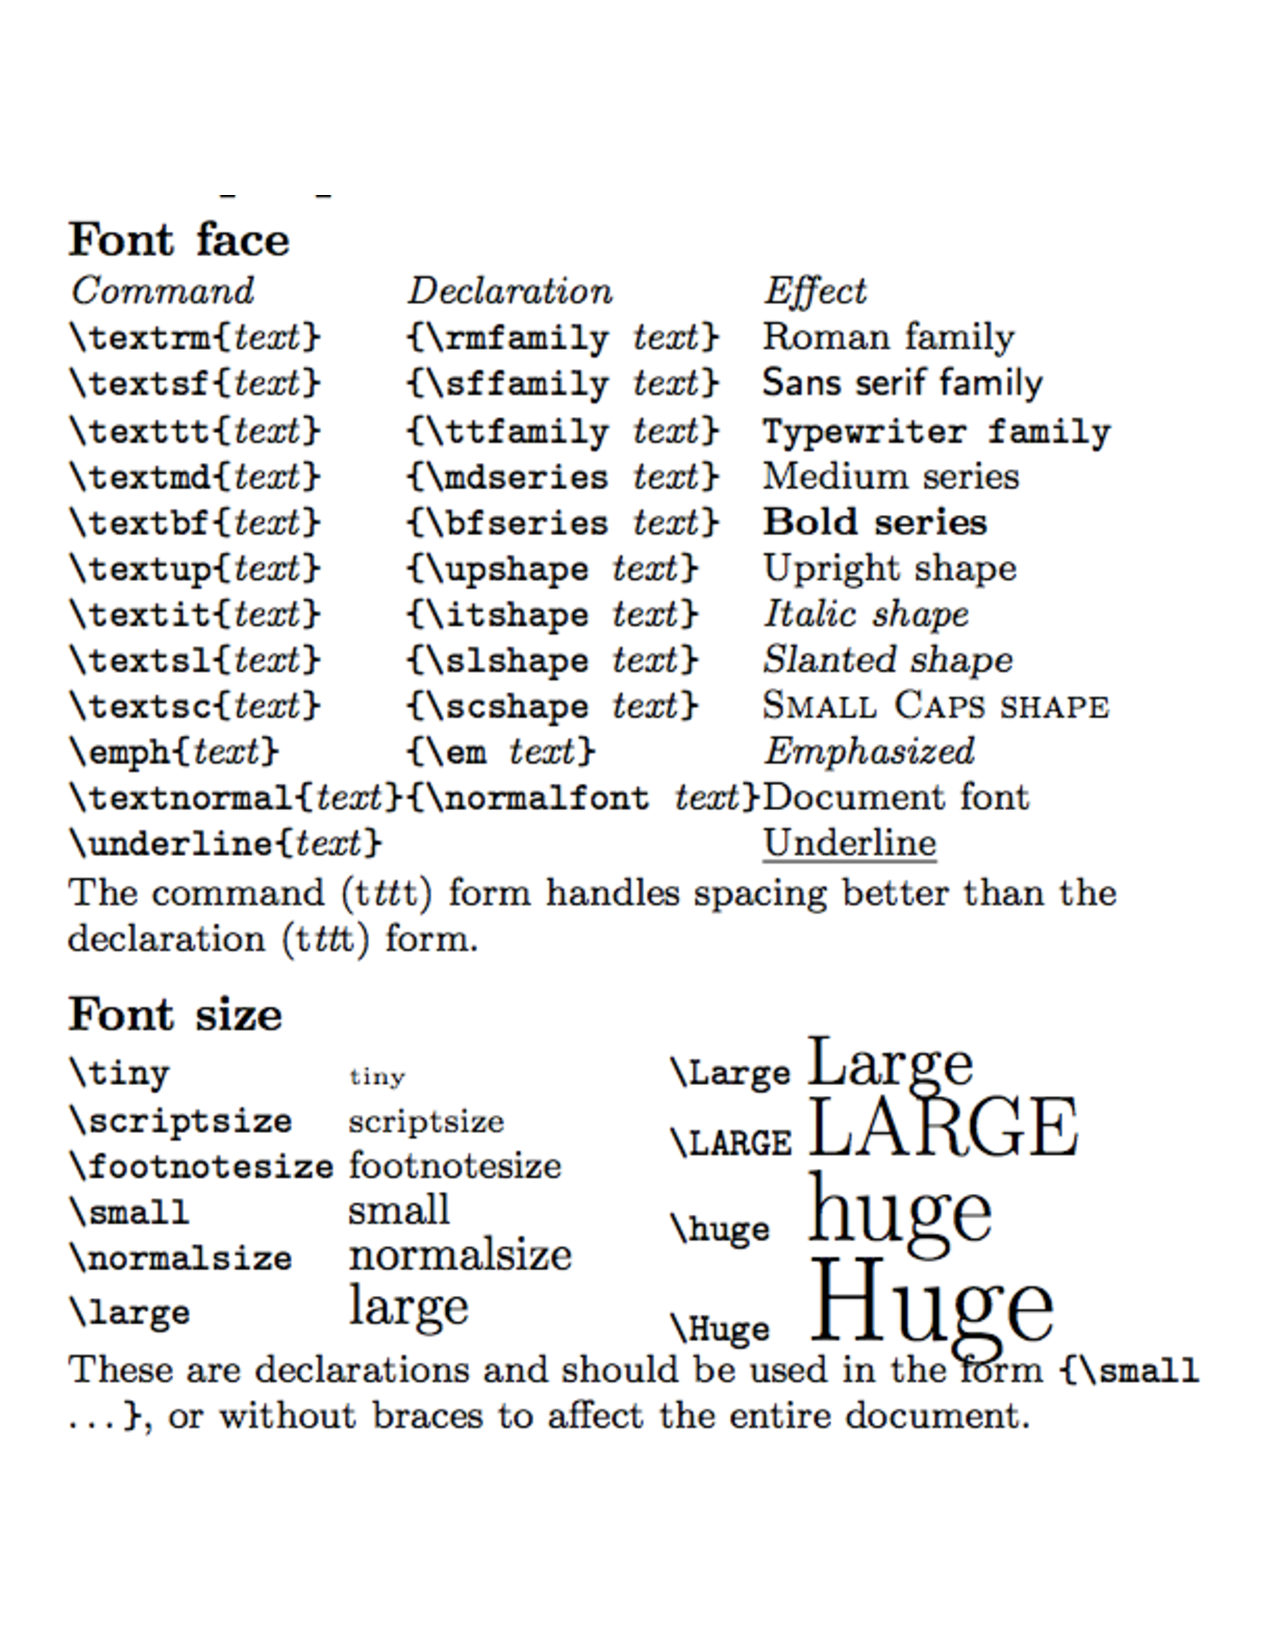
\includegraphics[scale=0.3]{figures/commands.pdf}\\
\end{frame}


\section{Figures, Tables, and Code}

% \begin{frame}[fragile]
% \frametitle{Working with \LaTeX\ and \texttt{R}: Tables}
% To avoid copy-pasting:
% \begin{itemize}
% \item<2->{Get \texttt{R} to write a \texttt{.tex} file for each table}
% \item<3->{Save the table in your w.d}
% \item<4->{Call that table using the ``$\backslash$include\{ \}'' command}
% \item<5->{Alternatively, use \texttt{sweave} or \texttt{knitr} or  \texttt{markup}.}
% \end{itemize}
% \end{frame}

\begin{frame}[fragile]
  \frametitle{Adding a figure or table}

  To insert figures in your document, include \verb+\usepackage{graphicx}+ in your preamble. Then

  \begin{lstlisting}
  \begin{figure}[hbt]
  \begin{center} % To keep the figure centered
  \includegraphics[scale=0.8]{figures/my_figure_filename}
  \end{center}
  \caption{A Pretty Plot}
  \end{figure}
  \end{lstlisting}
\end{frame}

\begin{frame}[fragile]
  \frametitle{Notes on figures and tables}
  \begin{itemize}
    \item You can specify the file extension, or not.
    \item The caption is also optional, but it's good practice to caption your figures and tables.
    \item Options for \verb+\includegraphics+ are e.g. \verb+[width=\textwidth]+ or \verb+[height=3cm]+
    \item Labels are also really useful! 	\verb+\label{tab:MyTab}+ combined with \verb+\ref{tab:MyTab}+
    \item Images should be in the same folder! (or \verb+\graphicspath{{Graphs/}}+)
    \item A useful \LaTeX{} table generator is \url{http://www.tablesgenerator.com/}
  \end{itemize}

\end{frame}


\begin{frame}
  \frametitle{Figure \& table environments: Floats}

  The positioning of
  floats can be frustrating if you don't know how they work or don't use
  the tools you have to control them.
  \begin{itemize}
    \item Every float has an optional positioning parameter:
          \texttt{\textbackslash begin\{figure\}[placement specifier]}.
    \item The default placement specifier, the one \LaTeX{} uses if we
          don't specify anything, is \texttt{tbp}, which stands for ``at the top of
          the page'', ``at the bottom of the page'', and ``at a special page
          containing only floats''.
          % \item When \LaTeX{} encounters a float, it tries to place
          %   it in the current place and if it can't, it puts it in a figures
          %   queue or in a tables queue, and every time it starts a new page, it
          %   tries to fill a special ``float page'' with floats from the
          %   queues. If it can't, it tries to place the first float in the
          %   queue. \LaTeX{} maintains the order in the queue.
    \item You can use other placement specificers, like ``h'' (for here),
          or ``!'' (which basically says ``override other parameters'').
    \item To avoid floats appearing outside the section where they belong
          (or say beyond a certain paragraph), you can use
          \texttt{\textbackslash FloatBarrier}.
  \end{itemize}
\end{frame}


\begin{frame}[fragile]
  \frametitle{Working with \LaTeX\ and \texttt{R}: Graphics}
  Normally you want to export R plots as PDF files (or EPS), not JPEG or PNG
  (unless you're dealing with a very large file like a map):
  \begin{columns}
    \begin{column}{.5\textwidth}
      R code:
      \begin{lstlisting}[basicstyle=\ttfamily\scriptsize]
    plot(rnorm, ylab=''Personal happiness'',
    xlab=''LaTeX ability'', lwd=3,
    col=''blue'')
    grid(lty=''dotted'')
  \end{lstlisting}
    \end{column}

    \begin{column}{.5\textwidth}
      \begin{center}
        Plot produced by R:
        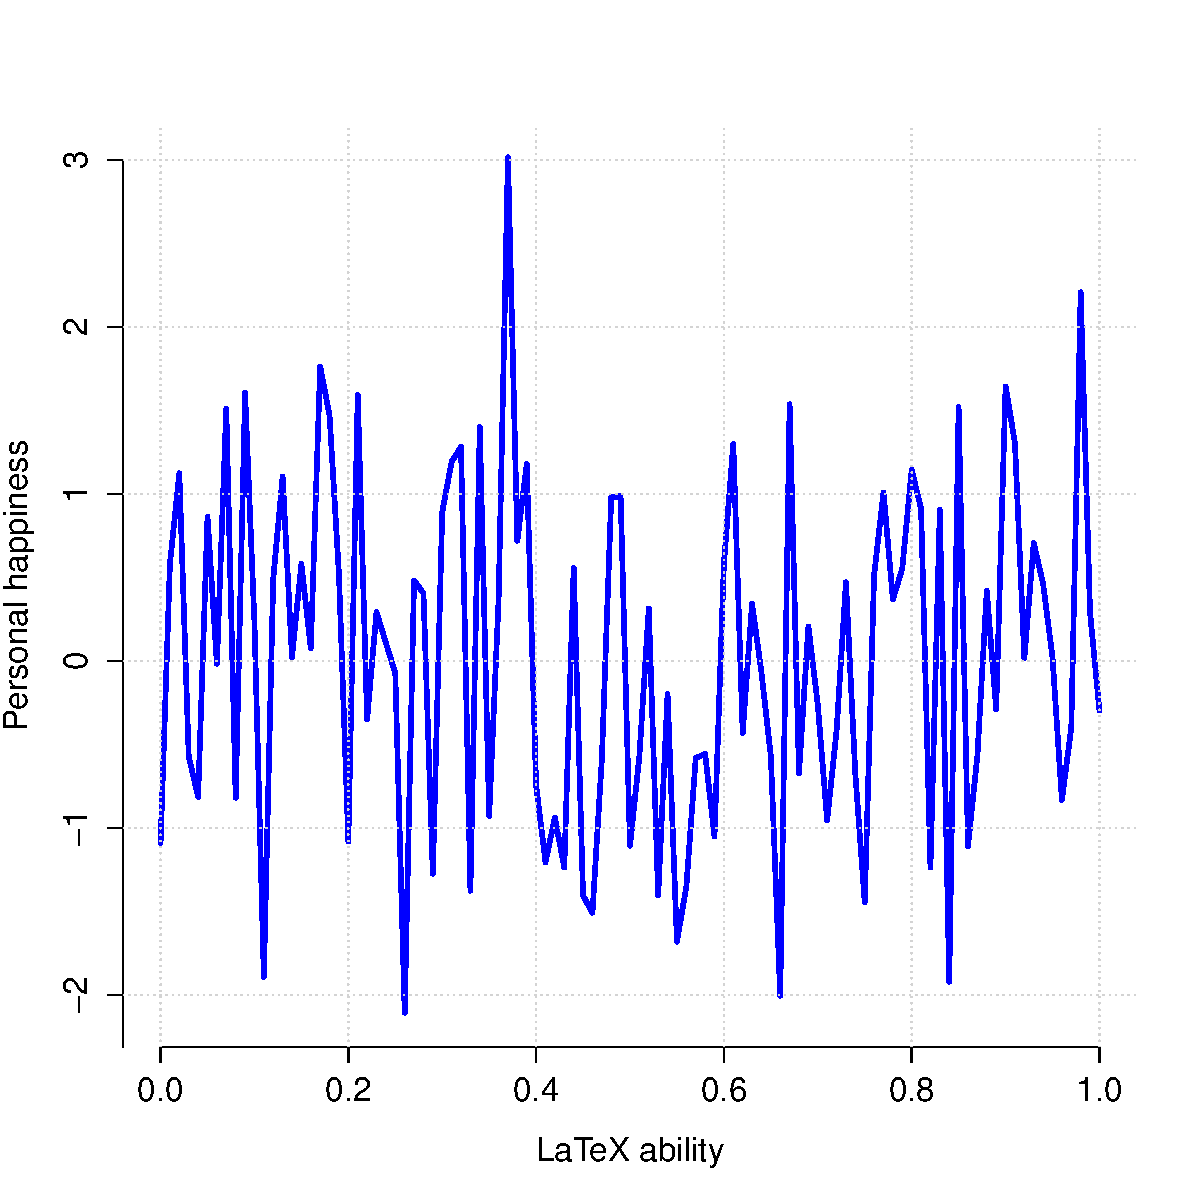
\includegraphics[scale=.25]{figures/fun.pdf}
      \end{center}
    \end{column}
  \end{columns}
\end{frame}

\begin{frame}[fragile]
  \frametitle{Working with \LaTeX\ and \texttt{R}: Tables}
  \begin{columns}
    \begin{column}{.48\textwidth}
      \begin{center}
        R code:
        \begin{lstlisting}
  mod1<-lm(y ~ x1 + x2)
  mod2<-lm(y ~ x1 * x2)
  stargazer(mod1, mod2)
  \end{lstlisting}
      \end{center}
      Note: \texttt{stargazer} is very flexible, and highly recommended for regression tables. \texttt{xtable} is a more generic function, will turn any matrix or data frame into a table.
    \end{column}

    \begin{column}{.48\textwidth}
      \begin{center}
        Output from \LaTeX: \\ \vspace{1em}
        \tiny{
          \begin{tabular}{@{\extracolsep{1pt}}lcc}
            \\[-1.8ex]\hline
            \hline                                                                                                  \\[-1.8ex]
                             & \multicolumn{2}{c}{\textit{Dependent variable:}}                                     \\
            \cline{2-3}
            \\[-1.8ex] & \multicolumn{2}{c}{y} \\
            \\[-1.8ex] & (1) & (2)\\
            \hline                                                                                                  \\[-1.8ex]
            x1               & 5.377$^{***}$                                                        & 4.922$^{***}$ \\
                             & (0.063)                                                              & (0.068)       \\
                             &                                                                      &               \\
            x2               & 5.916$^{***}$                                                        & 0.721         \\
                             & (0.318)                                                              & (0.618)       \\
                             &                                                                      &               \\
            x1:x2            &                                                                      & 1.043$^{***}$ \\
                             &                                                                      & (0.115)       \\
                             &                                                                      &               \\
            Constant         & $-$1.747$^{***}$                                                     & 0.450         \\
                             & (0.370)                                                              & (0.365)       \\
                             &                                                                      &               \\
            \hline                                                                                                  \\[-1.8ex]
            Observations     & 100                                                                  & 100           \\
            R$^{2}$          & 0.988                                                                & 0.993         \\
            Adjusted R$^{2}$ & 0.988                                                                & 0.993         \\
            \hline
            \hline                                                                                                  \\[-1.8ex]
            \textit{Note:}   & \multicolumn{2}{r}{$^{*}$p$<$0.1; $^{**}$p$<$0.05; $^{***}$p$<$0.01}                 \\
          \end{tabular}
        }
      \end{center}
    \end{column}%
  \end{columns}
\end{frame}


\begin{frame}[fragile]
  \frametitle{Working with \LaTeX\ and \texttt{R}: Code}
  When you want to import R-Code into your \LaTeX\ document, you have to use a special environment that allows the code to appear as is, with lines and special symbols intact. We recommend the \texttt{listings} package. To use, include \verb+\usepackage{listings}+ in your preamble, then type

  \begin{verbatim}
  \begin{lstlisting}
  Paste your R-Code, then...
  \end{lstlisting}
  \end{verbatim}

  In your preamble, you can adjust settings, e.g.

  \begin{lstlisting}
  \lstset{
  basicstyle=\ttfamily\footnotesize,  % font family/size
  breaklines=true                        % sets automatic line breaking
  }
  \end{lstlisting}

  Also: old-fashioned \verb+Verbatim+

\end{frame}

\begin{frame}
  \frametitle{Exercise: Export a graph and regression table into \LaTeX}
  \begin{enumerate}
    \item Open the \texttt{R} code file we sent you
    \item Run the graphing code in RStudio and export the graph as a pdf file.
    \item Run the \texttt{R} code to create data
    \item Run the \texttt{R} code that estimates models 1 and 2
    \item Using \texttt{stargazer}, export a regression table for both models
    \item Import the graph, the table, and the code into your \LaTeX\ document
  \end{enumerate}
\end{frame}

%-----------------------------------------------------------------------------

\section{Troubleshooting}

\begin{frame}
  \frametitle{What to do when things aren't working}

  Sometimes \LaTeX{} just won't compile, or compile and then delete the
  PDF file.

  \begin{itemize}
    \item Delete auxiliary files and compile again
    \item Think of what you edited since last time you successfully
          compiled your .tex file, and look at the code you added / edited -- the error
          must be there.
    \item Try googling your problem
    \item Check the .tex Stack exchange forum,
          and post a minimum working example if you can't find anything.
    \item Practice! Use \LaTeX{} to complete your problem sets for Quant I.
    \item Reach out to Quant I TAs for help.
          Feel free to post \LaTeX{} questions on Piazza,
          or raise them at recitation and/or office hours.
  \end{itemize}
\end{frame}


%-----------------------------------------------------------------------------

\section{Alternative \LaTeX{} Editors}
\begin{frame}
  \frametitle{Alternatives to TeXmaker}

  \begin{itemize}
    \item TeXworks (\href{https://www.tug.org/texworks/}{www.tug.org/texworks})
    \item TeXstudio (\href{https://www.texstudio.org/}{www.texstudio.org})
    \item Overleaf (\href{https://www.overleaf.com/}{www.overleaf.com})
    \item LyX (\href{https://www.lyx.org/}{www.lyx.org})
    \item Emacs (\href{https://www.gnu.org/software/emacs/}{www.gnu.org./software/emacs})

  \end{itemize}

\end{frame}

\begin{frame}
  \frametitle{The End?}

  Thank you!

\end{frame}

\appendix

\begin{frame}{Not Really!}

\end{frame}

\section{Reference management in \LaTeX{} using BibTeX}

\begin{frame}
  \frametitle{What is BibTeX and how does it work?}
  BibTeX, which is included in most TeX distributions, allows you to compile references throughout your .tex file, and to produce bibliographies automatically with pretty much any style you want.
  \begin{minipage}[b]{0.80\linewidth}
    \vspace{-10in}
    BibTeX is a compilation procedure for your \LaTeX\ code.
    \newline
    \newline
    \pause
    You run it in concert with the regular \LaTeX\ compiler.
    \newline
    \newline
    \pause
    One run of \LaTeX\, then BibTeX\, then \LaTeX\ twice...
    \newline
    \newline
    \pause
  \end{minipage}
  \begin{minipage}[b]{0.15\linewidth}

    \begin{center}
      (1)\LaTeX\\\ \pause $\Downarrow$ \\ (2)\alert{BibTeX}\ \pause $\Downarrow$ \\  (3)\LaTeX\\\ \pause $\Downarrow$ \\ (4)\LaTeX\\\ $\Downarrow$\\
      Voila!
    \end{center}
  \end{minipage}

  To use BibTex, we need to create a .bib file with our references in the correct format. Then we can "call" that file when compiling our .tex file.
\end{frame}

\begin{frame}[fragile]
  \frametitle{The ``.bib'' file}
  \begin{footnotesize}
    \begin{verbatim}
  @article{lipset1959,
    title={Some social requisites of democracy},
    author={Lipset, Seymour Martin},
    journal={American political science review},
    volume={53},
    number={1},
    pages={69--105},
    year={1959}
  }
  @book{dahl1973,
    title={Polyarchy: Participation and opposition},
    author={Dahl, Robert Alan},
    year={1973},
    publisher={Yale University Press}
  }
  \end{verbatim}
    Note that \texttt{lipset1959, dahl1973} are the (unique) keys, which we will use to cite it in our .tex file. You can directly get the formatted code for BibTeX references from Google Scholar, Zotero, etc.
  \end{footnotesize}
\end{frame}


\begin{frame}[fragile]
  \frametitle{Let's practice using BibTeX I}
  Add a new article to a .bib file:
  \begin{itemize}
    \item Open \texttt{practice.bib} in your \TeX\ editor
    \item Search for the article you want to include in Google scholar (or similar)
    \item Export the citation in BibTeX format (click ``cite''...)
    \item Copy the BibTeX\ format citation into \texttt{practice.bib}
    \item Change the \texttt{\alert{key}} to authorYEAR (or similar)
  \end{itemize}
\end{frame}

\begin{frame}[fragile]
  \frametitle{Let's practice using BibTeX II}
  Cite your new article and make a bibliography:
  \begin{itemize}
    \item Use the \texttt{natbib} package (Mac users may need package \texttt{cite} too)
    \item Create an inline citation using \verb+\citet{key}+
    \item Then a parenthetical citation with \verb+\citep{key}+
    \item Finally, include \verb+\bibliography{practice}+ and \verb+\bibliographystyle{chicago}+ at the bottom of your document
    \item Compile: \LaTeX\ $\rightarrow$ (2)\LaTeX\ $\rightarrow$  (3) BibTeX $\rightarrow$  (4)\LaTeX\ (or simply do ``Quick build'' in TeXMaker after you've configured it to do include BibTex compilation in Quick build going to texmaker > preferences > quick build).
  \end{itemize}
\end{frame}

\section{Referencing objects}

\begin{frame}[fragile]
  \frametitle{Labels \& references}
  Whenever you create a graph, table, or equation, you should label it.
  \begin{itemize}
    \item \textit{Equations}: Before you end your equation environment, include \verb+\label{eq_KEY}+
    \item \textit{Figures}: Wrap your figure in a \texttt{figure} environment, then include \verb+\label{fig_KEY}+ before \verb+\end{figure}+.  \verb+\label+ must be placed between \verb+\caption+ (if included) and \verb+\end{figure}+
    \item \textit{Tables}: As above.
  \end{itemize}
  To reference the equation, graph, or table in line, call the relevant label with \verb+\ref{fig_KEY}+
  \begin{itemize}
    \item \LaTeX{} will automatically order the objects of each type.%, giving you nicely numbered labels
    \item \verb+Figure~\ref{fig_KEY} shows blah blah blah+ \\
          $\Rightarrow$``Figure 7 shows blah blah blah''
    \item These will also sync with the captions you give to tables or
          graphs, which are also automatically numbered
    \item You can also label and reference sections, subsections etc.
  \end{itemize}
\end{frame}


\begin{frame}
  \frametitle{Exercise: Label and reference your graph and table}
  \begin{itemize}
    \item Make sure you use the right wrapper environments
    \item Use the \texttt{$\backslash$label} command
    \item Give appropriate labels to both objects
    \item Call the objects in-line
  \end{itemize}
\end{frame}

\section{Debugging}
\begin{frame}{Why is this not working???!}
  \begin{itemize}
    \item Did I make a typo?
    \item Have I forgotten a package in the preamble?
    \item Have I closed all the environments I have opened? \pause
    \item When was the last time this document compiled properly? \pause
    \item Google to the rescue!
  \end{itemize}
\end{frame}

\section{Internet friends!}

\begin{frame}{Internet resources that will make your life easier}
  \begin{itemize}
    \item \url{https://www.tablesgenerator.com/}
    \item Mathpix in action \pause
    \item Zotero export (not an internet friend, but an appreciated one)
  \end{itemize}

\end{frame}

\section{Presentations with \LaTeX}

\begin{frame}[fragile]{Getting started with Beamer}
  \begin{lstlisting}
	\documentclass{beamer}
	\end{lstlisting} \pause
  \begin{lstlisting}
	\begin{frame}{frame title}
		Text
	%\end{frame}
	\end{lstlisting}
  \pause
  \begin{lstlisting}
	\pause
	\end{lstlisting}
\end{frame}

\begin{frame}{Now let's try it!}
  \begin{itemize}
    \item Create a new document
    \item Set its class to \textit{beamer}
    \item Create a slide with a title
    \item Include some text (Maybe an itemized list?)
    \item Add some pauses in between the content of your slide
  \end{itemize}
\end{frame}

\begin{frame}[fragile]{Getting fancier I: Themes and customization}
  \begin{lstlisting}
\usetheme{CambridgeUS}
	\end{lstlisting} \pause
  Multiple themes available! Check: \url{https://deic-web.uab.cat/~iblanes/beamer_gallery/index.html}   \pause
  \begin{lstlisting}
\setbeamertemplate{navigation symbols}{}
\setbeamercolor{item projected}{bg=red}
	\end{lstlisting}
\end{frame}

\begin{frame}{Getting fancier II: Table of contents}
  \begin{itemize}
    \item Normal table of contents \pause
    \item And a fancier one
  \end{itemize}
\end{frame}


\end{document}
